\chapter{Appendix}
\section{$H_\infty$ Control Design} \label{app:hinf}
This control strategy consists in an optimization problem where the designer can specify a performance output to minimize; this minimization problem may be constructed in many possible ways by augmenting the plant with as many shaping function as the designer is willing to include.\\

In this scenario we decided to use the most common set-up given in the scheme depicted in figure \ref{fig:hinfscheme}. This scheme is valid for every scenario (number of degrees of freedom) described in this report, where $G(s)$ is the transfer function of the focus plant.\\

\begin{figure}[h]
	\centering
	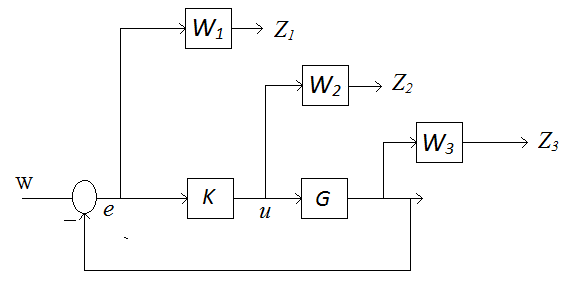
\includegraphics[width=0.5\textwidth]{img/hinf_scheme.png}
	\caption{Augmented plant. $G(s)$ represents the transfer function of the actuator and cart. $K(s)$ is the output controller of the $H_\infty$ minimization problem wrt the shaping functions $W_1(s), W_2(s), W_3(s)$.}
	\label{fig:hinfscheme}
\end{figure}

The minimization problem is stated as:
\begin{equation}
	\min_{W_1, W_2, W_3} 
		\begin{Vmatrix}
			z_1 \\ z_2 \\ z_3
		\end{Vmatrix}_\infty
	=
	\min_{W_1, W_2, W_3} 
		\begin{Vmatrix}
			S(s) W_1(s) \\ K(s) W_2(s) \\ T(s) W_3
		\end{Vmatrix}_\infty
\end{equation}
where, by letting $L(s) = K(s)G(s)$ be the openloop transfer function, the transfer functions $S, K, T$ are defined as
\begin{gather}
	S(s) = \frac{1}{1+L(s)} \\
	K(s)=\frac{K(s)}{1+L(s)} \\
	T(s)=\frac{L(s)}{1+L(s)}
\end{gather} 


\section{Effect of positive zeros}
Now it's briefly described what are the drawbacks of RHP-zeros in the loop. Essentialy what they do is, for an increasing number of positive zeros, to make the first $n$ derivatives of the output be $<0$ for $t=0$, except for those of order greater than $n$, $n>0$. This effect is well known for 1 positive zeros, where the first derivative is negative for $t=0$. For a pair of complex conjugate zeros from  a frequency analysis we can get an insight of what happens: they add  $-180$ degree to phase, therefore it's best to have those zeros at high frequency (thus the modulus of the zeros) to have their effect quickly dissipate without any effect. To analyze in time we need to take the partial 	fraction expansion. Let $G(s)$ be our system considered and $C(s)$ our controller. Then:
$$C(s) = \hat{k}\frac{(s-a)(s-\overline{a})}{s(s+p)}, a \in \mathbb{C}, p \in \mathbb{R}$$
where $\overline{a}$ is the complex conjugate of $a$, and $\hat{k}=\frac{kp}{|a|^2}$, with $\mathbb{R}(a) > 0$. 
The closed loop transfer function is:
$$T(s) = \frac{CG(s)}{1+CG(s)} = \frac{\hat{k}(s-a)(s-\overline{a})\gamma}{s(s+p)(Ls+R)(Ms^2+Cs+K)+\hat{k}(s-a)(s-\overline{a})\gamma}$$
With output signal $y(t) = \mathcal{L}[T(s)R(s)]^{-1}$.
For a certain $k$ it's possible to stabilize the system, that can be seen using root locus technique.
Notice that the motor since has a pole in $s \approx 600$ \SI{}{\radian \per \second} its term $sL$ can be ignored. In closed loop, it is possible to demonstrate that we have 2 complex conjugate poles in the left half plane, and two negative poles on the real axis that if the gain increases more will become complex conjugate poles. Thus we have 4 poles, and the transfer function can be rewritten as:
$$T(s) = \frac{\hat{k}(s-a)(s-\overline{a})\gamma}{(s+p_{1})(s+p_{2})(s^2+2\alpha s+\beta)}
$$
Where $p_2>p_1 >0 $. The partial fraction expansion becomes:
$$T(s) = \frac{A}{s+p_1} + \frac{B}{s+p_2} +\frac{Cs+D}{s^2+\alpha s+\beta}$$
and in time it's:
$$y(t) = Ae^{-p_1 t)}+ Be^{-p_2 t} +Ce^{-\alpha t}\Big (\cos(\theta t)+ \frac{\frac{D}{C}-\alpha}{\theta} \sin(\theta t) \Big)$$
Where $\theta^2 =  \beta -\alpha^2$. 
Making use of the fact that for example $A = \lim_{s \to -p_1} (s+p_1)T(s)$ we obtain:
\begin{align*}A &= \frac{\hat{k}(-p_1-a)(-p_1-\overline{a})\gamma}{(-p_1+p_2)(p_1^2-2\alpha p_1+\beta)}\\
B &= \frac{\hat{k}(-p_2-a)(-p_2-\overline{a})\gamma}{(-p_2+p_1)(p_2^2-2\alpha p_2+\beta)}
\end{align*}
And $$\lim_{t \to 0^{+}} \dot{y}(t) = \lim_{s \to \infty} sT(s) = A+B+C=0 \Rightarrow C=-A-B$$
$$T(0)= \frac{\hat{k}a^2\gamma}{p_1 p_2 \beta } = \frac{A}{p_1} + \frac{B}{p_2} + \frac{D}{\beta}$$
It can be proven that $\sign C =  - \sign \mathbb{R}(a)$, whilst $A,B,D$ mantain their sign. In fact $C$ is:
$$C=\frac{-\hat{k}\gamma}{p_2-p_1} \Big( \frac{(-p_1-a)(-p_1-\overline{a})}{p_1^2-2\alpha p_1+\beta} -\frac{(-p_2-a)(-p_2-\overline{a})}{p_2^2-2\alpha p_2+\beta} \Big) $$
Notice that the sign of $C$, with the hyphotesis $p_2 > p_1$, depends only on the numerator of the fractions inside the brackets (not the denominators, which are always positive):
$$C=\frac{-\hat{k}\gamma}{p_2-p_1}\Big ( \frac{p_1^2 -2p_1 \mathbb{R}(a) +a^2}{p_1^2-2\alpha p_1+\beta} -\frac{p_2^2 -2p_2 \mathbb{R}(a) +a^2}{p_2^2-2\alpha p_2+\beta} \Big)$$
For $\mathbb{R}(a) < 0 \Rightarrow C > 0$ and viceversa. This effects leads to $\dot{y}(t) <0$ for some $t$, causing the \emph{undershoot} effect.  \\ \\ \\
More in general, by looking at the expression of $T(s)$, it's possible to notice that the effect of $\mathbb{R}(a)$ is visible starting from the $r+1$ time derivative of $y(t)$, where $r$ is the relative degree, thus $\sign y^{r+1}(0)  = \sign \hat{k}\gamma \mathbb{R}(a)$. But derivative up to the $r$-th order are positive, thus for this reason the undershoot effect is delayed and does not appear right at the beginning. \\ \\
Finally an even number of positive zeros shows the undershoot effect  after a small time. On the other hand it can be proven  \cite{hoagg2006}]that an odd number of positive zeros shows the undershoot effect right at the start. Obviously the effect of those zeros can be reduced by moving them far away from the origin (i.e. in high frequency), where the gain of the system is very low,  but, then, the root locus would change. \\

\section{Extended Kalman Filtering}
Because of some problems with the Arduino Board with the continuous Kalman Filter we decided to use the discretized version of the Extended Kalman Filter.  To discretize the system the Forward Euler Method was used, therefore $\dot{x} \approx \frac{1}{t_s}(x_{n+1}-x_{n})$, where $t_s$ is the sampling time. Then, if the system in continuous time is described by the following equation:
\begin{equation}
\dot{x}=Ax+Bu
\end{equation}
In discrete time is:
\begin{equation}
x_{n+1}=(I+At_s)x_n + B t_s u
\end{equation}
Below is shown the matlab implementation of the algorithm:
\lstinputlisting{ekf.m}
